\documentclass[parskip=half]{scrartcl}

\usepackage[paperheight=3.5in, paperwidth=2.5in, margin=0.25in]{geometry}

\usepackage{fontspec}
\usepackage{enumitem}
\usepackage{caption}
\setmainfont{URWClassico}
\usepackage{tikz}

\definecolor{eruption_purple}{HTML}{513c3c}
\definecolor{eruption_pink}{HTML}{ff7280}

\setkomafont{section}{\setmainfont{LondrinaSolid}\Large\color{eruption_purple}}
\setkomafont{subsection}{\setmainfont{LondrinaSolid}\large\color{eruption_purple}}
\setkomafont{subsubsection}{\setmainfont{LondrinaSolid}\normalsize\color{eruption_purple}}

% Adjust spacing before and after section headings
\RedeclareSectionCommand[
  runin=false,
  beforeskip=0.5\baselineskip,
  afterskip=-0.0\baselineskip
]{section}

% Adjust spacing before and after subsection headings
\RedeclareSectionCommand[
  runin=false,
  beforeskip=0.5\baselineskip,
  afterskip=-0.0\baselineskip
]{subsection}

% Adjust spacing before and after subsubsection headings
\RedeclareSectionCommand[
  runin=false,
  beforeskip=0.5\baselineskip,
  afterskip=-0.0\baselineskip
]{subsubsection}

\tikzset{ring/.pic={
\pgfmathsetseed{#1} 

\foreach \i/\j in {0,72,...,359}
 \node[gray, fill=black, minimum width=3.5mm, minimum height=3.5mm, rotate=180*rand] at (\i:5mm) {};
 
\foreach \i/\j in {36,108,...,359}
 \node[gray, fill=black, minimum width=3.5mm, minimum height=3.5mm, rotate=180*rand] at (\i:7.5mm) {};

 \node[draw, black, very thick, fill=white, minimum width=3.5mm, minimum height=3.5mm, rotate=180*rand] at (0,0) {};

 \draw[ultra thick, brown] plot[smooth cycle,variable=\t,samples at={0,45,...,315}] (\t:rr);
}
}


\usepackage[hidelinks]{hyperref}

%\pagecolor{eruption_pink}
\begin{document}
\color{eruption_purple}
{
\enlargethispage{1.0\baselineskip}
\begin{center}
\setmainfont[Scale=1.0]{Earthquake MF} \Huge
ERUPTION

\setmainfont{URWClassico} \footnotesize
A dexterity game for 2\textendash{}6 players

\vfill

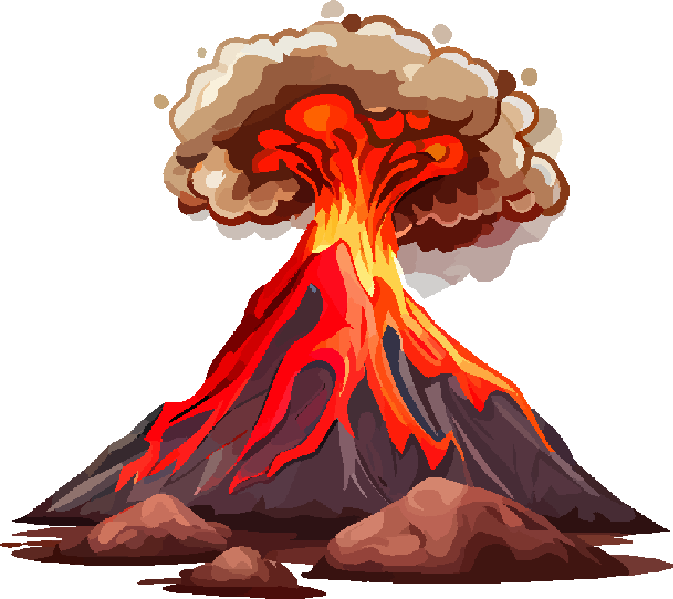
\includegraphics[width=2.0in]{Images/one_volcano.png}

\vfill

\setmainfont{URWClassico}
\normalsize
Designed by Michael Purcell
\end{center}
}

\newpage
\raggedright
\setmainfont{URWClassico} \small
\section*{Overview}
Eruption is a dexterity game for 2\textendash{}6 players. It can be played in about fifteen minutes and is intended for players who are at least twelve years old.

\section*{Components}
\begin{itemize}[leftmargin=*]
\item 175 wooden cubes (8mm)
\begin{itemize}[leftmargin=*]
\item 120 lava cubes (40 each of red, orange, and yellow)
\item 50 black cubes
\item 5 white cubes
\end{itemize}
\item 5 rubber bands (size \#31)
\end{itemize}

\newpage

\section*{Set Up}
\begin{enumerate}[leftmargin=*]
\item Choose one player to go first.

\item Each other player should place a rubber band \emph{volcano} in the middle of the play area.

\item Place ten black cubes and one white cube in each volcano.
\end{enumerate}

\vfill

\begin{figure}[hb]
\centering
%\begin{center}
\scalebox{0.55}{
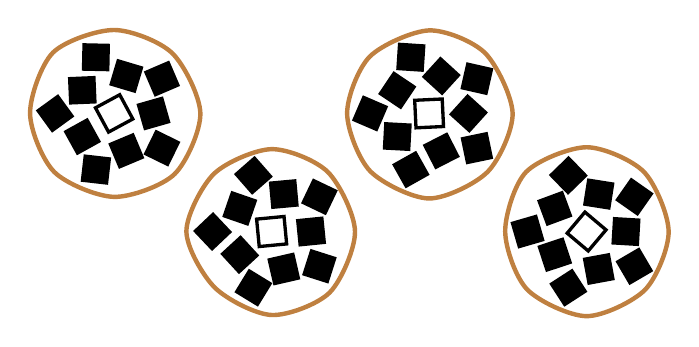
\begin{tikzpicture}[declare function={rr=1.0*(1+0.1*rnd);}]
\pic at (0,0) {ring={3}};

\pic at (6cm, -1.5cm) {ring={5}};

\pic at (2cm, -1.5cm) {ring={18}};

\pic at (4, 0cm) {ring={9}};
\end{tikzpicture}
}
%\end{center}
\caption*{{\scriptsize Setup for a five-player game.}}
\end{figure}
\newpage
\section*{Gameplay}
On your turn, place a lava cube into one of the volcanoes.
\begin{itemize}[leftmargin=*]
\item You must place your cube so that it is touching a white cube.
\item You may only use one hand at a time while placing your cube.
\end{itemize}

If any cubes fall out of a volcano, the volcano \emph{erupts}. If that happens during your turn, both you and the volcano are eliminated from the game.

You win if all of your opponents have been eliminated.

\newpage

\section*{Simultaneous Play (Optional)}
If you want a more frantic experience, you may choose to play a simultaneous game.

You will need a thirty-second timer in addition to the cubes and rubber bands.

\subsection*{Set Up}
\begin{enumerate}[leftmargin=*]
\item Each player should place a rubber-band volcano in front of themself.
\item Place the cubes within easy reach of all players.
\end{enumerate}

\subsection*{Gameplay}
First, start the timer. 

Then, try to place as many cubes into your volcano as possible before time expires. You may use only one hand to do so.

%If your volcano erupts, you are not eliminated. You may continue to play until time expires.

The game ends when time expires. You win if you have the most cubes in your volcano at the end of the game.  

\subsection*{Acknowledgement}
This simultaneous-play variant was suggested by Brett Witty.

\newpage

\section*{Two-Handed Play (Optional)}
If you have two or three players, you may choose to play a two-handed game.

\subsection*{Set Up}
Set up the game as if each hand is a separate player. 

\begin{itemize}[leftmargin=*]
\item For two players you should use three volcanoes.
\item For three players you should use five volcanoes.
\end{itemize}

\subsection*{Gameplay}
Play proceeds as normal except that you must alternate which hand you use on your turn.

If a volcano erupts on your turn, the hand you were using is eliminated. You may continue to play with your other hand.

You win if all of your opponents' hands have been eliminated.

\vfill
%\hrulefill

\scriptsize
\textbf{Design}: Michael Purcell\\
\textbf{Contact}: \href{mailto:ttkttkt@gmail.com}{ttkttkt@gmail.com}\\
\textbf{License}: This work is licensed under a\\\phantom{\textbf{License}: }``CC BY-SA 4.0'' license.%\raggedright\doclicenseText

\end{document}